\documentclass[%
    %handout
]{beamer}
\usepackage{graphicx} % For including single page pdfs
\usepackage{bm}       % bold math
\usepackage{pgffor}   % for loop
\usepackage{tikz}
\usepackage{multimedia}
\usepackage{layouts}
\usepackage{hyperref}
\usepackage{cambridge_lecture}
\usepackage{mathtools}
\newtheorem*{theorem*}{Theorem}


\title{Planck, inflation and the future of inflationary constraints}
\subtitle{Consistency of Cosmological Datasets: Evidence for new Physics?}
\author[Handley] % (optional, for multiple authors)
{Will Handley\\ \small{wh260@cam.ac.uk}}
\institute[University of Cambridge] % (optional)
{%
    Astrophysics Group \\
    Cavendish Laboratory \\
    University of Cambridge
}
\date{1\textsuperscript{st} June 2018}

\usepackage{calculator}

\newcommand{\cols}[3][0.5]{%
    \SUBTRACT{1.}{#1}{\wdthb}
    \begin{columns}
        \begin{column}{#1\textwidth}
            #2
        \end{column}
        \begin{column}{\wdthb\textwidth}
            #3
        \end{column}
    \end{columns}
}

\newcommand{\figname}{}
\newenvironment{figright}[2][0.5]{%
    \renewcommand{\figname}{#2}
    \SUBTRACT{1.}{#1}{\wdthb}
    \begin{columns}
        \begin{column}{#1\textwidth}
        }{%
        \end{column}
        \begin{column}{\wdthb\textwidth}
            \includegraphics[width=\textwidth]{\figname}
        \end{column}
    \end{columns}
}

\newcommand{\dfigname}{}
\newenvironment{dfigright}[3][0.5]{%
    \renewcommand{\figname}{#2}
    \renewcommand{\dfigname}{#3}
    \SUBTRACT{1.}{#1}{\wdthb}
    \begin{columns}
        \begin{column}{#1\textwidth}
        }{%
        \end{column}
        \begin{column}{\wdthb\textwidth}
            \includegraphics[width=\textwidth]{\figname}
            \includegraphics[width=\textwidth]{\dfigname}
        \end{column}
    \end{columns}
}



\newenvironment{figleft}[2][0.5]{%
    \SUBTRACT{1.}{#1}{\wdthb}
    \begin{columns}
        \begin{column}{#1\textwidth}
            \includegraphics[width=\textwidth]{#2}
        \end{column}
        \begin{column}{\wdthb\textwidth}
        }{%
        \end{column}
    \end{columns}
}

\newenvironment{dfigleft}[3][0.5]{%
    \SUBTRACT{1.}{#1}{\wdthb}
    \begin{columns}
        \begin{column}{#1\textwidth}
            \includegraphics[width=\textwidth]{#2}
            \includegraphics[width=\textwidth]{#3}
        \end{column}
        \begin{column}{\wdthb\textwidth}
        }{%
        \end{column}
    \end{columns}
}


\newcounter{numimages}

\newenvironment{multifig}[1]{%
    \begin{frame}
        \pdfximage{#1}%
        \setcounter{numimages}{\the\pdflastximagepages}
        \addtocounter{numimages}{-1}

        \begin{tikzpicture}[remember picture, overlay]
            \foreach \pagenum in {1,...,\thenumimages} {%
                \node<handout:0|beamer:\pagenum>[anchor=center] at (current page.center) {
                \includegraphics[width=\textwidth,page=\pagenum]{#1}}; 
            }
            \addtocounter{numimages}{1}
            \node<handout:1|beamer:\thenumimages>[anchor=center] at (current page.center) {
            \includegraphics[width=\textwidth,page=\thenumimages]{#1}}; 
        \end{tikzpicture}
    }{%
    \end{frame}
}


\begin{document}

\begin{frame}
    \titlepage{}
\end{frame}

\begin{frame}
    \frametitle{The pipeline from inflation to the CMB}
    \begin{columns}
        \begin{column}{0.5\textwidth}
            \centering
            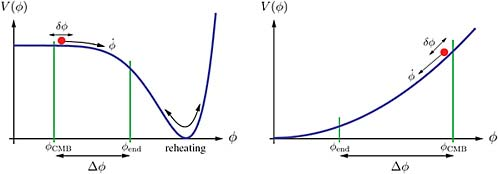
\includegraphics[width=\textwidth]{./figures/p2001dcd6g16001.jpg}
            \begin{minipage}{0.7\textwidth}
                
\begin{tikzpicture}
    % width of axes
    % length of crosses
    \def\croslen{0.1\textwidth}

    % Draw axes
    \draw [<->,thick] (0,0.5\textwidth) node (yaxis) [below right] {$\log\mathcal{P}_\mathcal{R}$}
    |- (\textwidth,0) node (xaxis) [above] {$\log k$};

    \coordinate (mn) at (0.1\textwidth,0.3\textwidth);
    \coordinate (mx) at (0.9\textwidth,0.25\textwidth);
    \draw (mn) -- (mx);
    \draw<1> (mx) node[below left] {$A_s {\left(\frac{k}{k_*}\right)}^{n_s-1}$};


\end{tikzpicture}


            \end{minipage}
            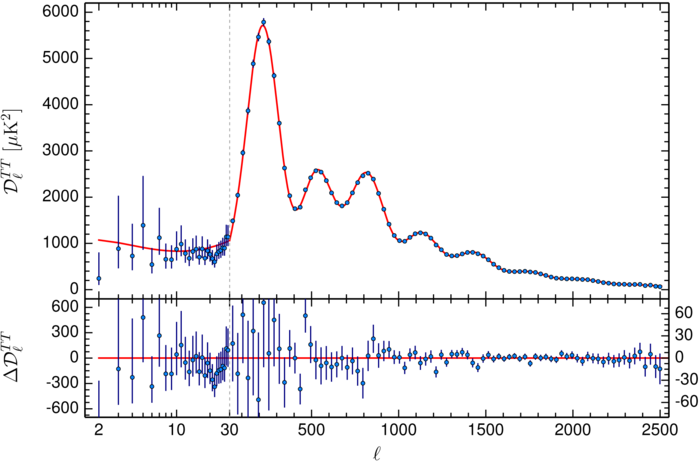
\includegraphics[width=0.7\textwidth]{./figures/700px-A15_TT.png}
        \end{column}
        \hfill
        \begin{column}{0.5\textwidth}
            \begin{itemize}
                \item Inflationary model
                \item Primordial power spectrum $\mathcal{P}_\mathcal{R}$
                \item $(A_s,n_s,r)$
                \item Boltzmann solver \& line-of-site projection
                \item $(\Omega_b h^2,\Omega_c h^2,\theta_\ast,\tau)$
                \item CMB power spectrum $C_\ell$
            \end{itemize}
        \end{column}
    \end{columns}

\end{frame}

\begin{frame}
    \frametitle{Constraining inflation (Planck 2015)}
    \framesubtitle{Linking theorists and observers}
    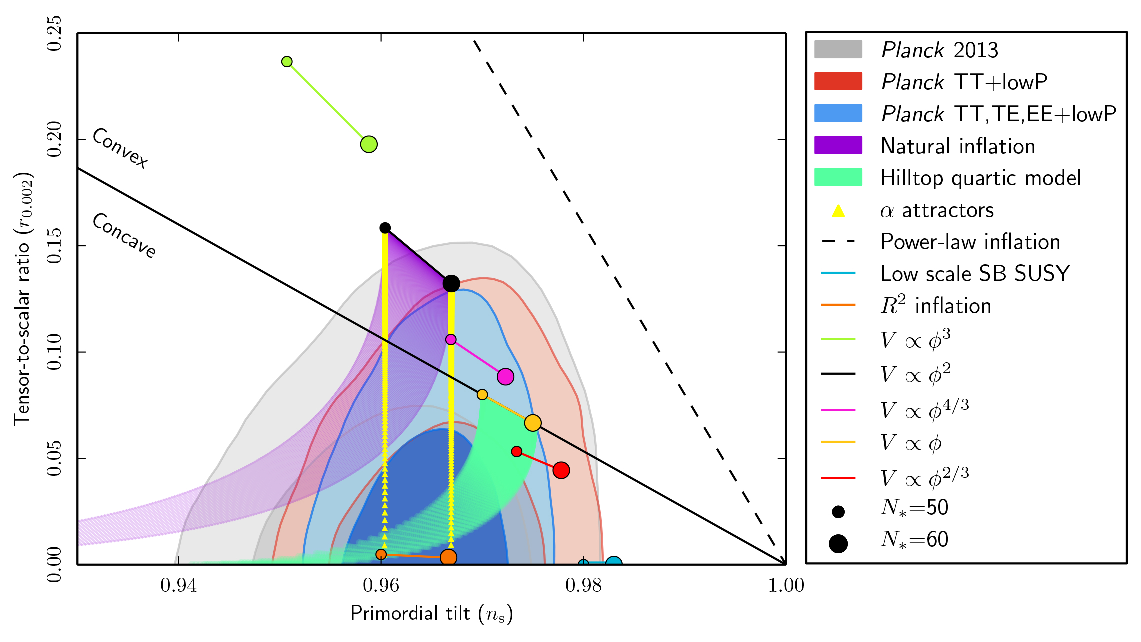
\includegraphics[width=\textwidth]{./figures/V18TTvsTTTEEEvs2013_120mmR.pdf}
\end{frame}


\begin{frame}
    \frametitle{COBE}
    \centering
    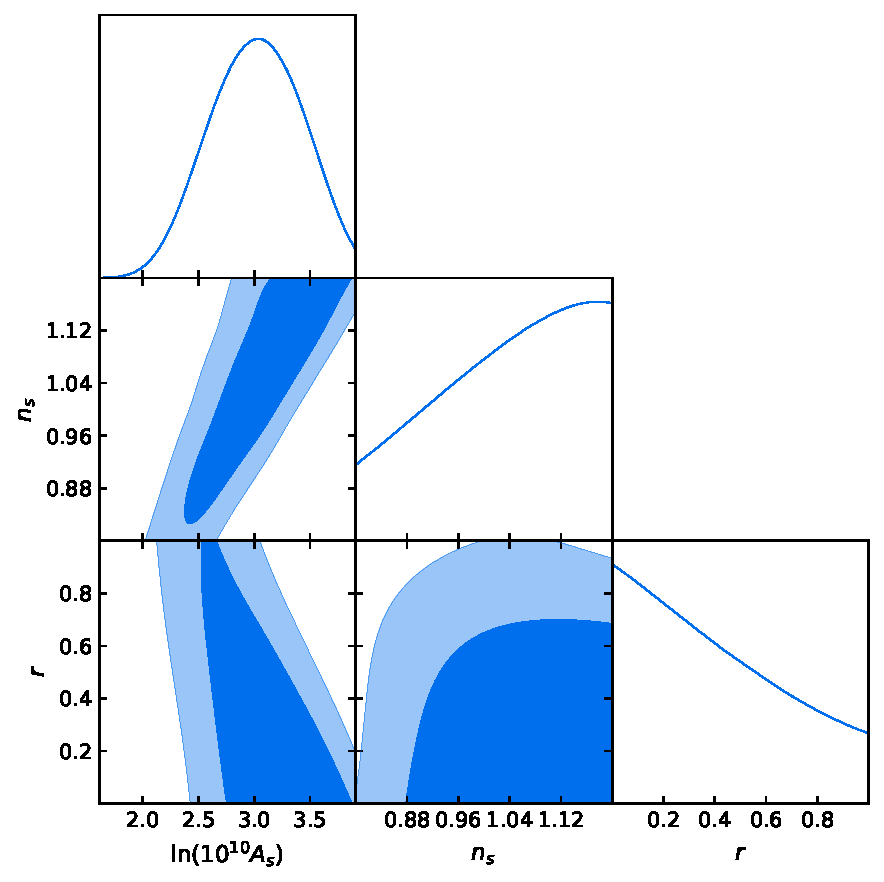
\includegraphics[width=0.7\textwidth]{./figures/COBE.pdf}
\end{frame}
\begin{frame}
    \frametitle{COBE, MAXIMA, BOOMERANG, VSA, DASI, CBI}
    \centering
    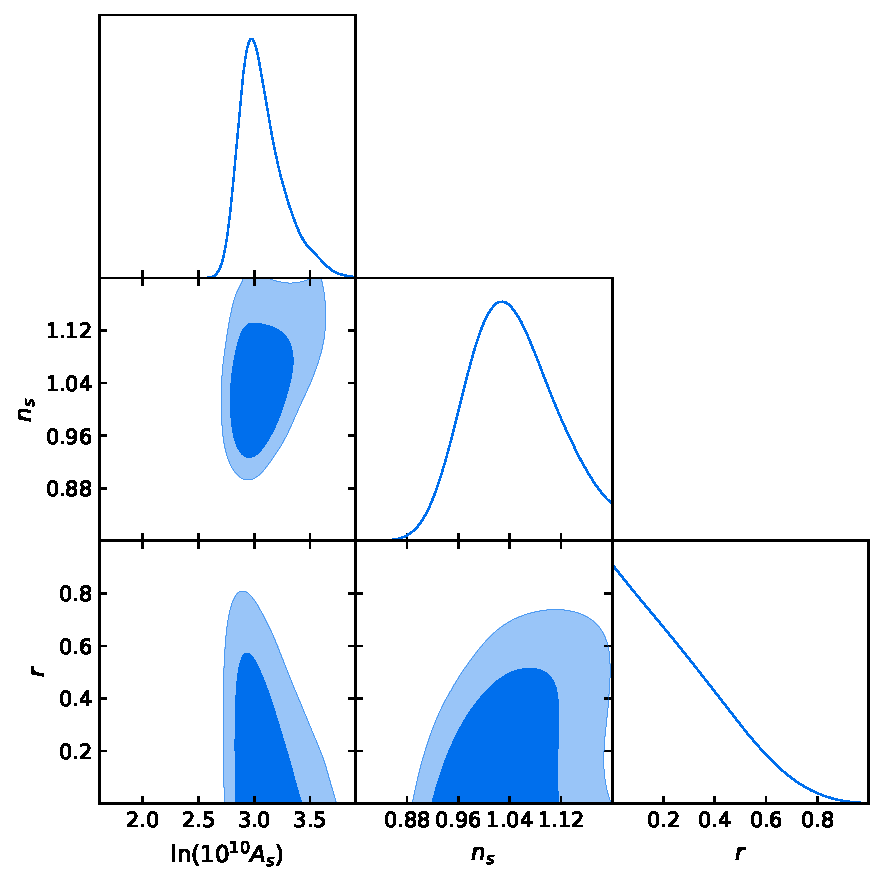
\includegraphics[width=0.7\textwidth]{./figures/pre_WMAP.pdf}
\end{frame}
\begin{frame}
    \frametitle{WMAP}
    \centering
    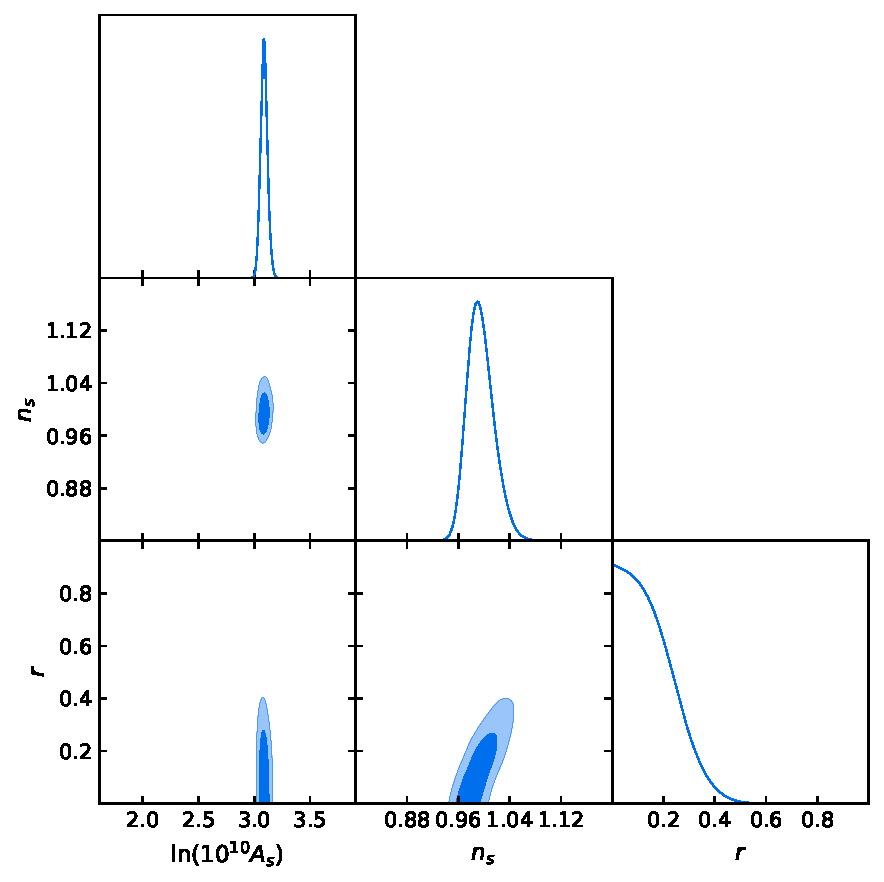
\includegraphics[width=0.7\textwidth]{./figures/WMAP.pdf}
\end{frame}
\begin{frame}
    \frametitle{Planck 2013}
    \centering
    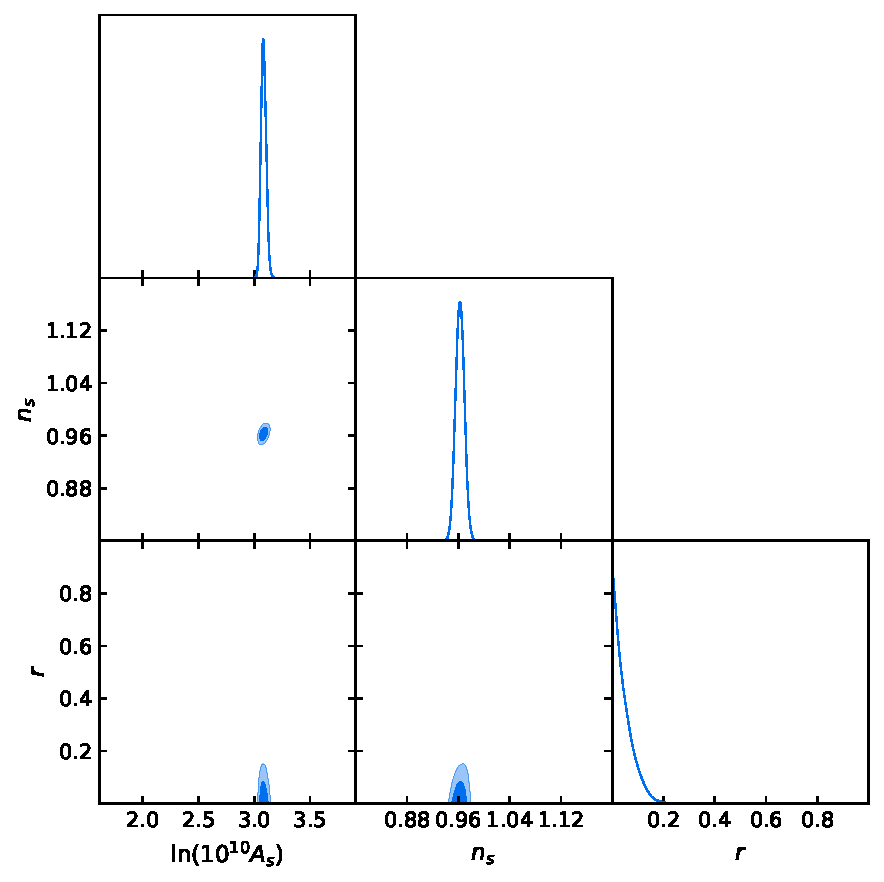
\includegraphics[width=0.7\textwidth]{./figures/planck_2013.pdf}
\end{frame}

\begin{frame}
    \frametitle{The Future}
    \centering
    \begin{figleft}[0.6]{./figures/combined.pdf}
        \begin{itemize}
            \item Lyth bound:  $r>0.01 \Rightarrow \Delta\phi > M_\mathrm{p}$
            \item LiteBird: $r\sim \mathcal{O}(10^{-3})$, $r\sim \mathcal{O}(N^{-2})$ $50<N<60$
            \item Compare specific inflationary models.
        \end{itemize}
    \end{figleft}
\end{frame}


\begin{frame}
    \frametitle{The importance of $\tau$}
    \centering
    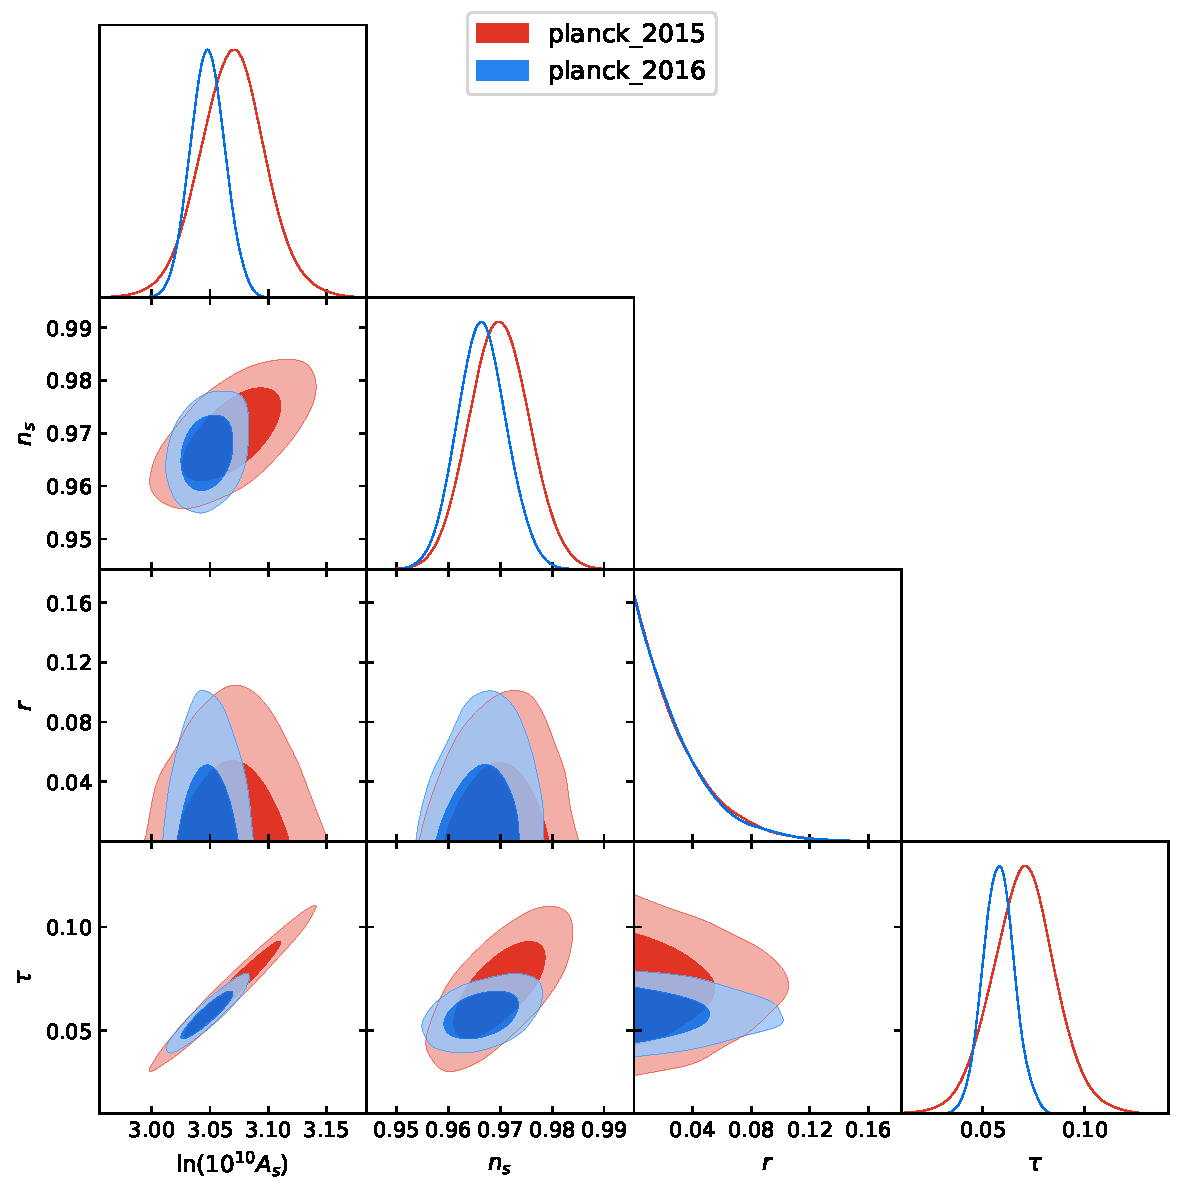
\includegraphics[width=0.7\textwidth]{./figures/tau_triangle_both.pdf}
\end{frame}

\begin{frame}
    \frametitle{Primordial power spectrum reconstruction}
    \centering
    \begin{minipage}{0.7\textwidth}
        
\begin{tikzpicture}
    % width of axes
    % length of crosses
    \def\croslen{0.1\textwidth}

    % Draw axes
    \draw [<->,thick] (0,0.67\textwidth) node (yaxis) [above] {$\log\mathcal{P}_\mathcal{R}$}
    |- (\textwidth,0) node (xaxis) [below] {$\log k$};

    \coordinate (mn) at (0.1\textwidth,0.4\textwidth);
    \coordinate (mx) at (0.9\textwidth,0.3\textwidth);
    \draw (mn) -- (mx);
    \draw<1> (mn) node[above right] {$A_s {\left(\frac{k}{k_*}\right)}^{n_s-1}$};


\end{tikzpicture}


    \end{minipage}
\end{frame}

\begin{frame}
    \frametitle{Primordial power spectrum reconstruction}
    \centering
    \begin{minipage}{0.7\textwidth}
        
\newcommand{\movablecross}[1]{%
    \draw[->](#1) -- ++(0:\croslen);
    \draw[->](#1) -- ++(90:\croslen);
    \draw[->](#1) -- ++(180:\croslen);
    \draw[->](#1) -- ++(270:\croslen);
    \fill[red!70!black] (#1) circle (2pt);
}

\newcommand{\movablevert}[1]{%
    \draw[->](#1) -- ++(90:\croslen);
    \draw[->](#1) -- ++(270:\croslen);
    \fill[red!70!black] (#1) circle (2pt);
}

\begin{tikzpicture}
    % width of axes
    % length of crosses
    \def\croslen{0.1\textwidth}


    % Draw axes
    \draw [<->,thick] (0,0.67\textwidth) node (yaxis) [above] {$\log\mathcal{P}_\mathcal{R}$}
    |- (\textwidth,0) node (xaxis) [below] {$\log k$};

    % Draw the line joining start and end
    \coordinate (mn) at (0.1\textwidth,0.3\textwidth);
    \coordinate (start) at (0.2\textwidth,0.6\textwidth);
    \coordinate (mid) at (0.5\textwidth,0.2\textwidth);
    \coordinate (end) at (0.6\textwidth,0.5\textwidth);
    \coordinate (mx) at (0.9\textwidth,0.4\textwidth);
    \draw (mn) node[below right]    {$(x_1,y_1)$};
    \draw (start) node[above right]     {$(x_2,y_2)$};
    \draw (mid) node[below right] {$(x_3,y_3)$};
    \draw (end) node[above right] {$(x_4,y_4)$};
    \draw (mx) node[below left]  {$(x_N,y_N)$};
    \movablevert{mn};
    \movablevert{mx};
    \movablecross{start};
    \movablecross{mid};
    \movablecross{end};

    \draw (mn) -- (start) -- (mid) -- (end) -- (mx);



\end{tikzpicture}


    \end{minipage}
\end{frame}

\begin{frame}
    \frametitle{Primordial power spectrum reconstruction with CORE}
    \centering
    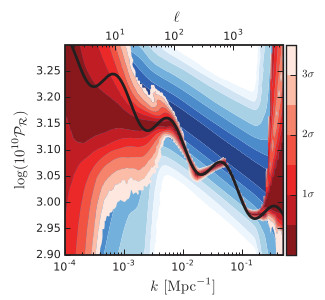
\includegraphics[width=0.49\textwidth]{./figures/posterior_monodromy_2.jpg}
    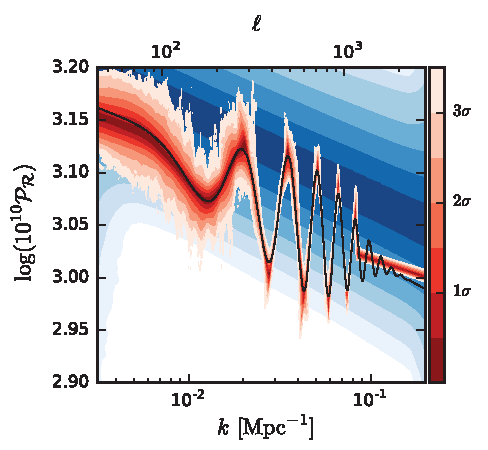
\includegraphics[width=0.49\textwidth]{./figures/posterior_cs_2.pdf}
\end{frame}

\begin{frame}
    \frametitle{The future of inflation observation}
    \centering
    \begin{figleft}[0.6]{./figures/pps.png}
        \begin{itemize}
            \item $r\stackrel{?}{\ne}0$ --- LiteBird
            \item better $\tau\Rightarrow$ feature finding --- CORE (CMB Bharat?) --- PICO?
            \item Spectral distortions --- PRISTINE?
            \item Alternative models to relieve tensions?
        \end{itemize}
    \end{figleft}
\end{frame}


\begin{frame}
    \frametitle{Alternative models: Kinetic dominance}
    \framesubtitle{``Just enough inflation''}
    \begin{figleft}[0.6]{./figures/wh293_100_v1.pdf}
        \begin{itemize}
            \item Only $\sim\mathcal{O}(60)$ efolds of total inflation 
            \item Preceded by generic phase of $\dot{\phi}^2\gg V(\phi)$
            \item Natural mechanism for generating low-$\ell$ supression
            \item Possibility of fitting $\ell\sim30$ feature
            \item Spatial curvature provides stronger justification.
        \end{itemize}
    \end{figleft}
\end{frame}

\begin{frame}
    \frametitle{The DES Bayes factor}
    \begin{figleft}[0.5]{./figures/Lahav_DES_DESI__Cambridge_29May2018.pdf}
        \begin{itemize}
            \item Contains everything it should, in a dimensionally consistent way:
                \begin{equation}
                    R = \frac{P(D_{pl},D_{des}|M)}{P(D_{pl}|M)P(D_{des}|M)}  \nonumber
                \end{equation}
            \item $R\sim 10$ default prior, $R\sim 0.1$ for narrower prior.
        \end{itemize}
        \begin{equation}
            R = \frac{P(D_{pl}|D_{des},M)}{P(D_{pl}|M)} = \frac{P(D_{pl}|M_{OL})}{P(D_{pl}|M_{GPE})} \nonumber
        \end{equation}
    \end{figleft}
    \begin{itemize}
        \item Represents Bayesian confidence in ability to combine the data
        \item The fact that there are physically reasonable priors which make $R<1$ means that as a Bayesian I am very suspicious of this combination.
        \item Conditioned on $\Lambda$CDM, these data are inconsistent.
    \end{itemize}
\end{frame}

%\begin{frame}
%    \frametitle{<++>}
%    \framesubtitle{<++>}
%
%	\begin{figright}{<++>}
%	\end{figright}
% 
%\end{frame}



\end{document}
